\documentclass[11pt,a4paper]{article}

\usepackage[utf8]{inputenc}
\usepackage[T1]{fontenc}
\usepackage[brazil]{babel}
\usepackage[margin=2.5cm]{geometry}
\usepackage{amsmath}
\usepackage{listings}
\usepackage{xcolor}
\usepackage{booktabs}
\usepackage{graphicx}
\usepackage[hidelinks]{hyperref}

\definecolor{fundo}{gray}{0.96}
\definecolor{comentario}{rgb}{0.25,0.45,0.25}
\definecolor{palavra}{rgb}{0.15,0.15,0.6}
\definecolor{textocor}{rgb}{0.6,0.2,0.2}

\lstdefinestyle{codigo}{
  backgroundcolor=\color{fundo},
  basicstyle=\ttfamily\small,
  commentstyle=\color{comentario}\itshape,
  keywordstyle=\color{palavra}\bfseries,
  stringstyle=\color{textocor},
  numbers=left,
  numberstyle=\tiny\color{gray},
  numbersep=8pt,
  frame=single,
  rulecolor=\color{gray},
  breaklines=true,
  showstringspaces=false,
  tabsize=2,
  captionpos=b,
  columns=fullflexible,
  keepspaces=true,
}
\lstset{style=codigo}

\title{Leitura do acelerômetro MPU6050 com ESP32\\[2mm]
       \large Explicação do código, bloco por bloco}
\author{Instrumentação Eletrônica para Engenharia --- Entrega 1}
\date{}

\begin{document}
\maketitle

\section*{Visão geral}

O projeto tem quatro arquivos e cada um resolve uma parte do problema. O
firmware lê o sensor e imprime números na porta serial. Um script em Python
pega esses números e salva em disco. Outro script transforma o arquivo salvo
no gráfico que a entrega pede. O quarto arquivo só diz ao PlatformIO qual é a
placa e qual biblioteca baixar.

\begin{center}
\begin{tabular}{@{}lll@{}}
\toprule
\textbf{Arquivo} & \textbf{Onde roda} & \textbf{O que faz} \\
\midrule
\texttt{platformio.ini} & computador  & configura a compilação \\
\texttt{src/main.cpp}   & ESP32       & lê o sensor e imprime CSV \\
\texttt{capturar.py}    & computador  & grava o CSV em arquivo \\
\texttt{plot\_dados.py} & computador  & desenha o gráfico \\
\bottomrule
\end{tabular}
\end{center}

O caminho do dado é sempre o mesmo: o MPU6050 mede, manda por I2C para a
ESP32, a ESP32 converte e manda por USB para o computador, o Python grava e
depois plota.

\vspace{3mm}
\noindent
Ordem de uso:

\begin{enumerate}
  \item \texttt{pio run -t upload} grava o firmware na placa.
  \item \texttt{python capturar.py} faz o ensaio e salva \texttt{dados.csv}.
  \item \texttt{python plot\_dados.py} gera \texttt{grafico.png}.
\end{enumerate}

\newpage
\section{Bloco 1 --- \texttt{platformio.ini}}

\begin{lstlisting}[caption={platformio.ini}]
[env:esp32doit-devkit-v1]
platform = espressif32
board = esp32doit-devkit-v1
framework = arduino

monitor_speed = 115200

lib_deps =
    electroniccats/MPU6050@^1.3.1

upload_port  = COM3
monitor_port = COM3
\end{lstlisting}

Esse arquivo não é código, é receita. O PlatformIO lê cada linha e decide o
que baixar e como compilar.

\texttt{platform} escolhe a família do chip e traz junto o compilador
\texttt{xtensa}, que gera código para o processador da ESP32. São centenas de
megabytes, baixados uma vez só, na primeira compilação.

\texttt{board} é o modelo exato da placa. Define quanta flash existe, qual o
cristal, e o mapa de pinos. Trocar essa linha muda o binário gerado.

\texttt{framework = arduino} é o que permite escrever \texttt{setup()},
\texttt{loop()}, \texttt{Serial.print()} e \texttt{delay()}. Sem ele o
programa teria que ser escrito com as funções do ESP-IDF, que são bem mais
verbosas.

\texttt{lib\_deps} é a única dependência do projeto. O PlatformIO baixa a
biblioteca MPU6050 da Electronic Cats direto do registro dele e a coloca em
\texttt{.pio/libdeps/}. O \texttt{\^{}1.3.1} aceita qualquer versão 1.x a
partir da 1.3.1, mas nunca a 2.0, que poderia quebrar a interface.

As duas últimas linhas fixam a porta COM3. Sem elas o PlatformIO tenta
adivinhar, e quando há mais de um dispositivo USB-serial ligado ele erra.

\newpage
\section{Bloco 2 --- \texttt{src/main.cpp} (37 linhas)}

Esse é o firmware inteiro. Ele faz três coisas: acorda o sensor, lê os três
eixos, imprime. Nada mais.

\subsection{Includes (linhas 1--3)}

\begin{lstlisting}[language=C++,firstnumber=1]
#include <Arduino.h>
#include <Wire.h>
#include <MPU6050.h>
\end{lstlisting}

\texttt{Arduino.h} traz \texttt{setup()}, \texttt{loop()}, \texttt{Serial},
\texttt{delay()} e \texttt{millis()}. Na IDE do Arduino esse include é
automático; no PlatformIO, que compila \texttt{.cpp} de verdade, ele precisa
estar escrito.

\texttt{Wire.h} é a biblioteca de I2C. O MPU6050 fala I2C, e é por aqui que a
comunicação acontece.

\texttt{MPU6050.h} é a biblioteca do sensor. Ela já inclui internamente o
\texttt{I2Cdev}, que é a camada que lê e escreve os registradores.

\subsection{Pinos (linhas 5--6)}

\begin{lstlisting}[language=C++,firstnumber=5]
#define SDA_PIN 21
#define SCL_PIN 22
\end{lstlisting}

Na DevKit v1 os pinos 21 e 22 são os de I2C por padrão. SDA carrega os dados,
SCL carrega o clock. Usar \texttt{\#define} em vez de escrever 21 e 22 soltos
no meio do código deixa claro o que cada número significa, e se a ligação
mudar basta editar aqui.

\subsection{A constante 16384 (linhas 8--9)}

\begin{lstlisting}[language=C++,firstnumber=8]
// na faixa de +-2g o sensor entrega 16384 contagens por g
#define LSB_POR_G 16384.0
\end{lstlisting}

Esse número não foi escolhido, ele sai da conta. O conversor
analógico-digital do MPU6050 tem 16 bits com sinal, ou seja, o valor lido vai
de $-32768$ a $+32767$. Na faixa de $\pm 2$\,g essa escala inteira representa
4\,g de ponta a ponta. Logo:

\[
\frac{32768}{2\ \mathrm{g}} = 16384 \ \text{contagens por g}
\]

O ponto zero no final (\texttt{16384.0}) é o detalhe que mais derruba gente em
C. Se estivesse escrito \texttt{16384}, o compilador trataria como inteiro, e
\texttt{ax / LSB\_POR\_G} viraria divisão inteira: uma leitura de 16400
contagens daria 1 em vez de 1{,}001, e tudo abaixo de 16384 daria 0. Com o
\texttt{.0} a constante é um \texttt{double}, o \texttt{int16\_t} é promovido,
e a divisão sai em ponto flutuante.

\subsection{O objeto do sensor (linha 11)}

\begin{lstlisting}[language=C++,firstnumber=11]
MPU6050 mpu;
\end{lstlisting}

Cria o objeto que representa o sensor. O construtor sem argumento assume o
endereço I2C \texttt{0x68}, que é o endereço quando o pino AD0 do módulo está
em GND ou solto. Se o AD0 for ligado em 3V3 o endereço vira \texttt{0x69} e a
linha teria que ser \texttt{MPU6050 mpu(0x69);}.

\subsection{A função \texttt{setup()} (linhas 13--22)}

\begin{lstlisting}[language=C++,firstnumber=13]
void setup() {
  Serial.begin(115200);
  delay(2000);

  Wire.begin(SDA_PIN, SCL_PIN);
  mpu.initialize();
  mpu.setFullScaleAccelRange(MPU6050_ACCEL_FS_2);

  Serial.println("t_ms,ax_g,ay_g,az_g");
}
\end{lstlisting}

O \texttt{setup()} roda uma vez, logo depois que a placa liga ou reseta.

\textbf{Linha 14.} Abre a porta serial a 115200 bits por segundo. Esse número
aparece em três lugares do projeto e os três têm que bater: aqui, no
\texttt{monitor\_speed} do \texttt{platformio.ini}, e no \texttt{ser.baudrate}
do \texttt{capturar.py}. Se um deles divergir, o resultado é texto embaralhado
na tela.

\textbf{Linha 15.} Dois segundos parados. Parece desperdício, mas o conversor
USB-serial da placa leva um tempo para o Windows reconhecer a porta depois do
reset. Sem essa espera, as primeiras linhas impressas se perdem, incluindo o
cabeçalho do CSV.

\textbf{Linha 17.} Liga o barramento I2C com a ESP32 como mestre. A frequência
padrão é 100\,kHz, folgada para jumper de protoboard.

\textbf{Linha 18.} A linha mais importante do arquivo. Quando o MPU6050 é
alimentado ele acorda em modo de suspensão: o bit \texttt{SLEEP} do
registrador \texttt{PWR\_MGMT\_1} vem em 1 de fábrica, e nesse estado todas as
leituras voltam zeradas. O \texttt{initialize()} zera esse bit, escolhe a
fonte de clock e deixa o sensor medindo. Esquecer essa chamada é o erro mais
comum de quem começa com esse sensor: o código compila, roda, não dá erro
nenhum, e os três eixos ficam parados em zero.

\textbf{Linha 19.} Fixa a faixa em $\pm 2$\,g. É a faixa com melhor resolução
(61\,$\mu$g por contagem) e a certa para medir gravidade, que nunca passa de
1\,g. Para medir impacto ou vibração forte seria preciso subir para
$\pm 8$\,g ou $\pm 16$\,g, e aí o \texttt{LSB\_POR\_G} da linha 9 teria que
mudar junto.

\textbf{Linha 21.} Imprime o cabeçalho do CSV. É a primeira linha do arquivo e
serve para quem abrir no Excel saber o que é cada coluna.

\subsection{A função \texttt{loop()} (linhas 24--37)}

\begin{lstlisting}[language=C++,firstnumber=24]
void loop() {
  int16_t ax, ay, az;
  mpu.getAcceleration(&ax, &ay, &az);

  Serial.print(millis());
  Serial.print(",");
  Serial.print(ax / LSB_POR_G, 4);
  Serial.print(",");
  Serial.print(ay / LSB_POR_G, 4);
  Serial.print(",");
  Serial.println(az / LSB_POR_G, 4);

  delay(50);
}
\end{lstlisting}

O \texttt{loop()} roda para sempre, repetindo enquanto a placa estiver ligada.

\textbf{Linha 25.} Três variáveis de 16 bits com sinal. O tipo foi escolhido
para casar exatamente com o que o sensor devolve: nem maior, nem menor.

\textbf{Linha 26.} Faz a leitura. A função lê seis registradores de uma vez
(de \texttt{0x3B} a \texttt{0x40}), junta os bytes alto e baixo de cada eixo e
guarda o resultado. O \texttt{\&} antes de cada variável passa o endereço dela
na memória, e é isso que permite a função escrever em três variáveis de uma
vez só, coisa que um \texttt{return} normal não faria.

\textbf{Linhas 28--34.} Montam a linha do CSV. O \texttt{millis()} devolve
quantos milissegundos se passaram desde que a placa ligou, e vira a coluna de
tempo. Cada valor bruto é dividido por 16384 para virar g. O segundo
argumento do \texttt{Serial.print}, o número 4, é a quantidade de casas
decimais. A última chamada é \texttt{println} em vez de \texttt{print}, e é
ela que fecha a linha com a quebra que o Python vai usar para separar as
amostras.

\textbf{Linha 36.} Espera 50\,ms antes de repetir, o que dá mais ou menos 20
amostras por segundo. Medindo os tempos no arquivo gerado, o intervalo real
fica em torno de 51{,}6\,ms, porque a leitura I2C e a impressão também
consomem tempo e o \texttt{delay} só conta a partir do fim delas. A taxa
efetiva é de aproximadamente 19{,}4\,Hz. Para esse ensaio a diferença não
importa, já que o tempo verdadeiro de cada amostra vai gravado na primeira
coluna.

\subsection{O que o firmware não faz}

Vale registrar o que ficou de fora de propósito, porque a entrega pede só a
leitura do acelerômetro:

\begin{itemize}
  \item não lê o giroscópio, embora o chip tenha um;
  \item não faz calibração nem desconta offset;
  \item não aplica filtro de nenhum tipo, os valores são crus;
  \item não verifica se o sensor respondeu.
\end{itemize}

O último item tem consequência prática. Se o cabo estiver solto, o programa
continua imprimindo, só que com todos os eixos em zero. O sintoma de falha é
esse, e não uma mensagem de erro.

\newpage
\section{Bloco 3 --- \texttt{capturar.py} (46 linhas)}

Esse script existe por um motivo específico. O jeito óbvio de salvar os dados
seria \texttt{pio device monitor > dados.csv}, mas o PlatformIO recusa
redirecionamento de saída, e mesmo quando funcionava o PowerShell gravava o
arquivo em UTF-16 com os avisos do PlatformIO misturados no meio. Ler a porta
direto com a biblioteca \texttt{pyserial} resolve os dois problemas de uma
vez.

\subsection{Argumentos (linhas 8--9)}

\begin{lstlisting}[language=Python,firstnumber=8]
porta = sys.argv[1] if len(sys.argv) > 1 else "COM3"
saida = sys.argv[2] if len(sys.argv) > 2 else "dados.csv"
\end{lstlisting}

\texttt{sys.argv} é a lista do que foi digitado na linha de comando. O
\texttt{sys.argv[0]} é o nome do script, o \texttt{[1]} é o primeiro
argumento, e assim por diante. Rodando \texttt{python capturar.py} sem nada, o
script usa COM3 e \texttt{dados.csv}. Rodando
\texttt{python capturar.py COM5 ensaio.csv}, ele usa o que foi passado.

\subsection{Abrir a porta sem resetar errado (linhas 11--19)}

\begin{lstlisting}[language=Python,firstnumber=11]
# O DTR e o RTS dessa placa vao no GPIO0 e no EN. Se o pyserial ativar
# os dois na abertura, a ESP32 cai em modo de gravacao e nao envia nada.
ser = serial.Serial()
ser.port = porta
ser.baudrate = 115200
ser.timeout = 1
ser.dtr = False
ser.rts = False
ser.open()
\end{lstlisting}

Esse é o trecho menos óbvio do projeto inteiro, e vale entender direito.

A ESP32 precisa de dois sinais para ser gravada: o EN, que reseta o chip, e o
GPIO0, que decide se o boot é normal ou se entra no gravador. Para não
obrigar o usuário a apertar botão toda vez, as placas DevKit trazem um par de
transistores que liga o DTR e o RTS do conversor USB-serial nesses dois pinos.

O problema é que o \texttt{pyserial}, quando abre a porta do jeito normal
(\texttt{serial.Serial("COM3", 115200)}), ativa DTR e RTS juntos. Essa
combinação é exatamente a que joga a placa em modo de gravação. Foi o que
aconteceu no primeiro teste: a porta abria, a leitura rodava, e não vinha
nenhum byte.

A solução está na ordem das linhas. Criar o objeto sem passar a porta (linha
13) não abre nada. Os parâmetros são preenchidos um a um, o DTR e o RTS são
postos em \texttt{False}, e só depois o \texttt{open()} é chamado. A porta
abre com os dois sinais já desligados.

\subsection{O pulso de reset (linhas 21--25)}

\begin{lstlisting}[language=Python,firstnumber=21]
# pulso no EN para a placa reiniciar e a captura comecar do inicio
ser.rts = True
time.sleep(0.1)
ser.rts = False
ser.reset_input_buffer()
\end{lstlisting}

Com o DTR desligado, o GPIO0 fica em nível alto, que é a condição de boot
normal. Mexer só no RTS reseta a placa sem risco de cair no gravador.

O RTS vai para \texttt{True}, o que puxa o EN para baixo e segura o chip em
reset. Cem milissegundos depois o RTS volta para \texttt{False}, o EN sobe, e
a placa reinicia rodando o firmware. O \texttt{reset\_input\_buffer()} joga
fora o que já tinha chegado, para a captura começar limpa.

O ganho disso é que cada execução do script começa com o \texttt{millis()}
zerado na placa. Sem o reset, o tempo da primeira amostra seria um número
qualquer, dependendo de há quanto tempo a placa estava ligada.

\subsection{O laço de leitura (linhas 32--42)}

\begin{lstlisting}[language=Python,firstnumber=32]
try:
    while True:
        linha = ser.readline().decode(errors="replace").strip()
        if linha.count(",") != 3:   # descarta as mensagens de boot da ESP32
            continue
        arquivo.write(linha + "\n")
        arquivo.flush()
        n += 1
        print(n, linha, end="      \r")
except KeyboardInterrupt:
    pass
\end{lstlisting}

\textbf{Linha 34.} O \texttt{readline()} espera até chegar uma quebra de
linha, ou até estourar o \texttt{timeout} de 1 segundo. O que volta são bytes
crus, e o \texttt{decode} transforma em texto. O \texttt{errors="replace"}
evita que um byte corrompido derrube o programa no meio do ensaio. O
\texttt{strip()} tira a quebra de linha do fim.

\textbf{Linha 35.} O filtro. Toda linha válida do firmware tem exatamente três
vírgulas, porque tem quatro campos. As mensagens que o bootloader da ESP32
imprime ao ligar não seguem esse formato: a linha
\texttt{rst:0x1 (POWERON\_RESET),boot:0x13 (...)} tem uma vírgula, e a linha
\texttt{clk\_drv:0x00,q\_drv:0x00,...} tem cinco. Contar vírgula é o teste
mais barato que separa as duas coisas. O cabeçalho
\texttt{t\_ms,ax\_g,ay\_g,az\_g} passa no teste, e é isso que se quer: ele
fica gravado como primeira linha do arquivo.

\textbf{Linhas 37--38.} Escreve e força a gravação em disco na hora. Sem o
\texttt{flush()}, o Python guardaria vários kilobytes em memória antes de
escrever, e um Ctrl+C no momento errado perderia o fim do ensaio.

\textbf{Linha 40.} O argumento \texttt{end} termina com o caractere
\texttt{\textbackslash r}, que faz o cursor voltar para o começo da linha em
vez de pular para a próxima. O resultado é um contador que se atualiza no
mesmo lugar da tela, em vez de rolar centenas de linhas. Os espaços antes dele
apagam o resto de uma linha anterior que tenha sido mais comprida.

\textbf{Linhas 41--42.} Ctrl+C no terminal levanta a exceção
\texttt{KeyboardInterrupt}. Capturando ela aqui, o script sai do laço em vez
de morrer com um traceback feio, e ainda dá tempo de fechar o arquivo e a
porta nas linhas seguintes.

\newpage
\section{Bloco 4 --- \texttt{plot\_dados.py} (51 linhas)}

\subsection{Leitura do arquivo (linhas 14--29)}

\begin{lstlisting}[language=Python,firstnumber=14]
for linha in open(arquivo):
    campos = linha.strip().split(",")
    if len(campos) != 4:
        continue
    try:
        ms = int(campos[0])
        gx = float(campos[1])
        gy = float(campos[2])
        gz = float(campos[3])
    except ValueError:
        continue   # pula a linha do cabecalho

    t.append(ms / 1000.0)
    x.append(gx)
    y.append(gy)
    z.append(gz)
\end{lstlisting}

Percorrer o arquivo com \texttt{for linha in open(...)} lê uma linha por vez,
sem carregar tudo na memória.

O \texttt{split(",")} quebra a linha nas vírgulas e devolve uma lista de
pedaços. A verificação de tamanho descarta qualquer linha que não tenha
exatamente quatro campos.

O \texttt{try} resolve o cabeçalho sem precisar de uma regra especial para
ele. Quando o Python tenta fazer \texttt{int("t\_ms")}, ele levanta
\texttt{ValueError}, o \texttt{except} captura, e a linha é pulada. Uma linha
truncada por um cabo desconectado no meio da captura cai no mesmo lugar.

A ordem importa. Os quatro valores são convertidos primeiro para variáveis
soltas, e só depois de os quatro darem certo é que entram nas listas. Se a
conversão fosse feita direto dentro do \texttt{append}, uma linha que falhasse
no terceiro campo já teria deixado o tempo e o X gravados, e as quatro listas
ficariam com tamanhos diferentes. O gráfico sairia deslocado sem avisar.

\subsection{Tempo relativo (linhas 34--35)}

\begin{lstlisting}[language=Python,firstnumber=34]
inicio = t[0]
t = [v - inicio for v in t]
\end{lstlisting}

A primeira amostra chega com uns 2 segundos no relógio, por causa do
\texttt{delay(2000)} do firmware. Subtrair o valor inicial de todos faz o
gráfico começar em zero, que é como se espera ler um ensaio.

\subsection{O gráfico (linhas 37--51)}

\begin{lstlisting}[language=Python,firstnumber=41]
plt.axhline(1.0, color="gray", linestyle="--", linewidth=0.8)
plt.axhline(0.0, color="gray", linestyle="--", linewidth=0.8)
plt.axhline(-1.0, color="gray", linestyle="--", linewidth=0.8)
\end{lstlisting}

As três linhas tracejadas em $-1$, 0 e $+1$\,g são o gabarito visual do
ensaio. Com o sensor parado, cada curva tem que pousar em cima de uma delas.
Qualquer desvio visível já é erro de medida, e fica fácil de apontar no
relatório.

O \texttt{savefig} vem antes do \texttt{show}, e essa ordem não é acidental:
em vários backends do matplotlib a janela interativa esvazia a figura ao ser
fechada, e um \texttt{savefig} depois disso gravaria uma imagem em branco.

\newpage
\section{Bloco 5 --- O ensaio}

O enunciado pede a leitura com o sensor em posições coincidentes com o vetor
da gravidade. São seis posições, uma para cada sentido dos três eixos. Com o
sensor parado, o eixo que estiver na vertical marca $\pm 1$\,g e os outros
dois ficam perto de zero.

\begin{center}
\begin{tabular}{@{}lccc@{}}
\toprule
\textbf{Posição do módulo} & \textbf{X (g)} & \textbf{Y (g)} & \textbf{Z (g)} \\
\midrule
deitado, componentes para cima    & 0    & 0    & $+1$ \\
deitado, de cabeça para baixo     & 0    & 0    & $-1$ \\
de pé sobre a borda, X para baixo & $+1$ & 0    & 0 \\
borda oposta, X para cima         & $-1$ & 0    & 0 \\
de pé sobre a borda, Y para baixo & 0    & $+1$ & 0 \\
borda oposta, Y para cima         & 0    & $-1$ & 0 \\
\bottomrule
\end{tabular}
\end{center}

O procedimento é rodar o \texttt{capturar.py}, segurar cada posição por uns
cinco segundos, passar devagar de uma para a outra, e encerrar com Ctrl+C. Os
trechos parados viram patamares no gráfico e os movimentos viram os
transitórios entre eles.

\begin{figure}[h]
\centering
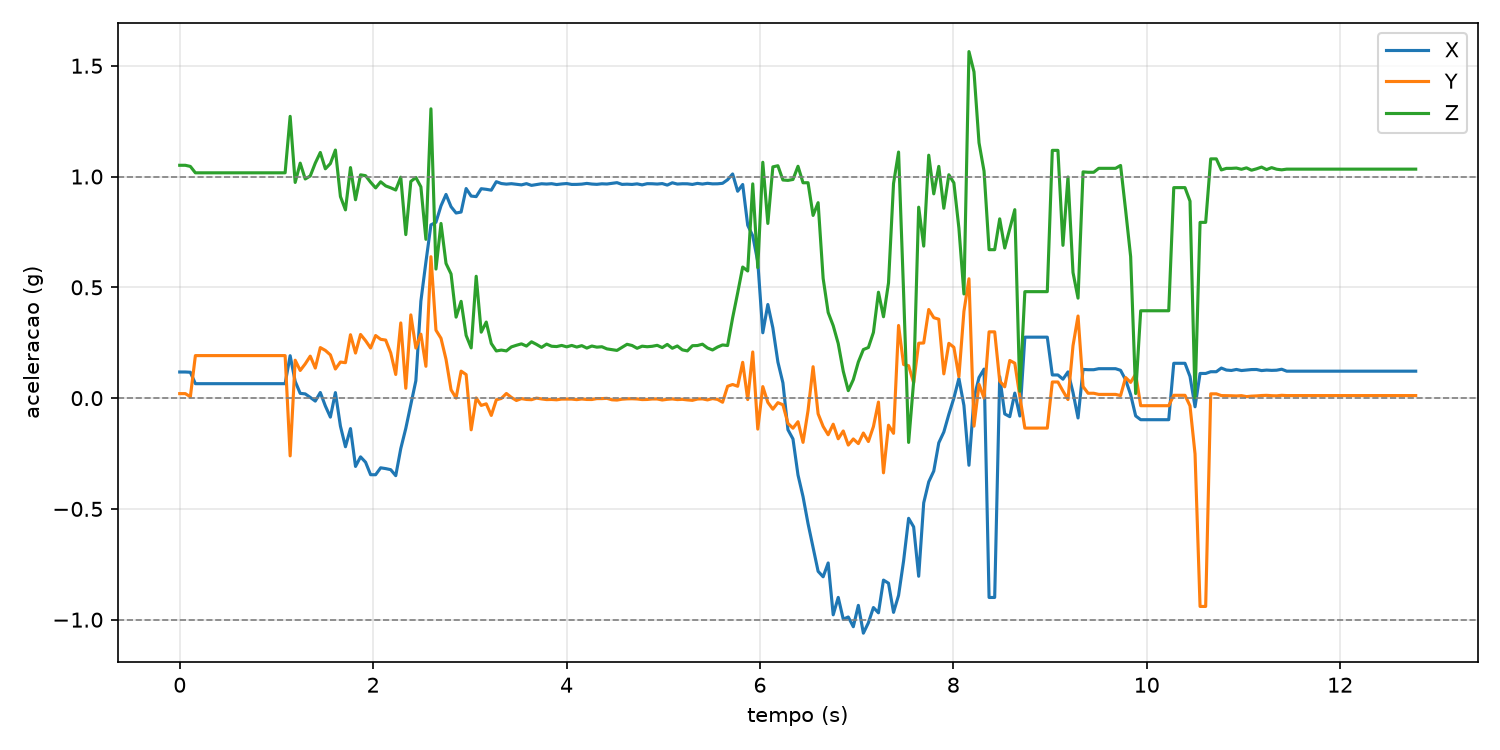
\includegraphics[width=\textwidth]{grafico.png}
\caption{Captura de exemplo. Os patamares em $+1$\,g de Z no início e de X no
fim correspondem a duas das seis posições da tabela; a agitação no meio é a
transição feita à mão.}
\end{figure}

\newpage
\section{Limitações conhecidas}

Essas são as coisas que o código não resolve, e que valem ser citadas no
relatório como fontes de erro.

\paragraph{O chip não é um MPU6050.} O registrador \texttt{WHO\_AM\_I}
respondeu \texttt{0x70}, que corresponde a um MPU6500. É um clone muito comum
nos módulos GY-521 vendidos hoje. Os registradores do acelerômetro são os
mesmos, por isso o código funciona sem alteração, mas as características de
ruído e as faixas do filtro interno são diferentes das do datasheet do
MPU6050. A tabela do item 2 deveria citar o datasheet do MPU6500.

\paragraph{Não há calibração.} Com a protoboard parada sobre a mesa, o eixo X
marcou em torno de $+0{,}12$\,g em vez de zero. Parte disso é inclinação real
da mesa e parte é o erro de offset de fábrica, que o datasheet especifica em
até $\pm 80$\,mg. Separar as duas contribuições exigiria nivelar o sensor com
bolha e repetir a medida em posições opostas.

\paragraph{A amostragem não é rigorosamente periódica.} O \texttt{delay(50)}
garante um intervalo mínimo, não um intervalo exato. O período medido ficou em
51{,}6\,ms. Para uma análise no domínio da frequência isso seria um problema,
e a solução correta seria disparar a leitura por interrupção de timer.

\paragraph{A faixa de $\pm 2$\,g satura.} Numa captura em que o módulo foi
sacudido de propósito, os picos ficaram ceifados em exatamente 2{,}00\,g. O
valor não é o real, é o teto da escala. Para medir impacto seria preciso
trocar a faixa na linha 19 do firmware e ajustar o \texttt{LSB\_POR\_G} da
linha 9.

\paragraph{O script assume COM3.} A porta está escrita direto no código como
valor padrão. Em outro computador, ou até nessa máquina com outro dispositivo
USB ligado antes, o número muda. O jeito de contornar é passar a porta como
argumento.

\end{document}
